% Options for packages loaded elsewhere
\PassOptionsToPackage{unicode}{hyperref}
\PassOptionsToPackage{hyphens}{url}
\PassOptionsToPackage{dvipsnames,svgnames,x11names}{xcolor}
%
\documentclass[
  11pt,
  a4paper,
  DIV=11,
  numbers=noendperiod]{scrartcl}

\usepackage{amsmath,amssymb}
\usepackage{iftex}
\ifPDFTeX
  \usepackage[T1]{fontenc}
  \usepackage[utf8]{inputenc}
  \usepackage{textcomp} % provide euro and other symbols
\else % if luatex or xetex
  \usepackage{unicode-math}
  \defaultfontfeatures{Scale=MatchLowercase}
  \defaultfontfeatures[\rmfamily]{Ligatures=TeX,Scale=1}
\fi
\usepackage{lmodern}
\ifPDFTeX\else  
    % xetex/luatex font selection
\fi
% Use upquote if available, for straight quotes in verbatim environments
\IfFileExists{upquote.sty}{\usepackage{upquote}}{}
\IfFileExists{microtype.sty}{% use microtype if available
  \usepackage[]{microtype}
  \UseMicrotypeSet[protrusion]{basicmath} % disable protrusion for tt fonts
}{}
\makeatletter
\@ifundefined{KOMAClassName}{% if non-KOMA class
  \IfFileExists{parskip.sty}{%
    \usepackage{parskip}
  }{% else
    \setlength{\parindent}{0pt}
    \setlength{\parskip}{6pt plus 2pt minus 1pt}}
}{% if KOMA class
  \KOMAoptions{parskip=half}}
\makeatother
\usepackage{xcolor}
\usepackage[lmargin=2cm,rmargin=2cm,tmargin=2cm,bmargin=2cm]{geometry}
\setlength{\emergencystretch}{3em} % prevent overfull lines
\setcounter{secnumdepth}{-\maxdimen} % remove section numbering
% Make \paragraph and \subparagraph free-standing
\ifx\paragraph\undefined\else
  \let\oldparagraph\paragraph
  \renewcommand{\paragraph}[1]{\oldparagraph{#1}\mbox{}}
\fi
\ifx\subparagraph\undefined\else
  \let\oldsubparagraph\subparagraph
  \renewcommand{\subparagraph}[1]{\oldsubparagraph{#1}\mbox{}}
\fi

\usepackage{color}
\usepackage{fancyvrb}
\newcommand{\VerbBar}{|}
\newcommand{\VERB}{\Verb[commandchars=\\\{\}]}
\DefineVerbatimEnvironment{Highlighting}{Verbatim}{commandchars=\\\{\}}
% Add ',fontsize=\small' for more characters per line
\usepackage{framed}
\definecolor{shadecolor}{RGB}{241,243,245}
\newenvironment{Shaded}{\begin{snugshade}}{\end{snugshade}}
\newcommand{\AlertTok}[1]{\textcolor[rgb]{0.68,0.00,0.00}{#1}}
\newcommand{\AnnotationTok}[1]{\textcolor[rgb]{0.37,0.37,0.37}{#1}}
\newcommand{\AttributeTok}[1]{\textcolor[rgb]{0.40,0.45,0.13}{#1}}
\newcommand{\BaseNTok}[1]{\textcolor[rgb]{0.68,0.00,0.00}{#1}}
\newcommand{\BuiltInTok}[1]{\textcolor[rgb]{0.00,0.23,0.31}{#1}}
\newcommand{\CharTok}[1]{\textcolor[rgb]{0.13,0.47,0.30}{#1}}
\newcommand{\CommentTok}[1]{\textcolor[rgb]{0.37,0.37,0.37}{#1}}
\newcommand{\CommentVarTok}[1]{\textcolor[rgb]{0.37,0.37,0.37}{\textit{#1}}}
\newcommand{\ConstantTok}[1]{\textcolor[rgb]{0.56,0.35,0.01}{#1}}
\newcommand{\ControlFlowTok}[1]{\textcolor[rgb]{0.00,0.23,0.31}{#1}}
\newcommand{\DataTypeTok}[1]{\textcolor[rgb]{0.68,0.00,0.00}{#1}}
\newcommand{\DecValTok}[1]{\textcolor[rgb]{0.68,0.00,0.00}{#1}}
\newcommand{\DocumentationTok}[1]{\textcolor[rgb]{0.37,0.37,0.37}{\textit{#1}}}
\newcommand{\ErrorTok}[1]{\textcolor[rgb]{0.68,0.00,0.00}{#1}}
\newcommand{\ExtensionTok}[1]{\textcolor[rgb]{0.00,0.23,0.31}{#1}}
\newcommand{\FloatTok}[1]{\textcolor[rgb]{0.68,0.00,0.00}{#1}}
\newcommand{\FunctionTok}[1]{\textcolor[rgb]{0.28,0.35,0.67}{#1}}
\newcommand{\ImportTok}[1]{\textcolor[rgb]{0.00,0.46,0.62}{#1}}
\newcommand{\InformationTok}[1]{\textcolor[rgb]{0.37,0.37,0.37}{#1}}
\newcommand{\KeywordTok}[1]{\textcolor[rgb]{0.00,0.23,0.31}{#1}}
\newcommand{\NormalTok}[1]{\textcolor[rgb]{0.00,0.23,0.31}{#1}}
\newcommand{\OperatorTok}[1]{\textcolor[rgb]{0.37,0.37,0.37}{#1}}
\newcommand{\OtherTok}[1]{\textcolor[rgb]{0.00,0.23,0.31}{#1}}
\newcommand{\PreprocessorTok}[1]{\textcolor[rgb]{0.68,0.00,0.00}{#1}}
\newcommand{\RegionMarkerTok}[1]{\textcolor[rgb]{0.00,0.23,0.31}{#1}}
\newcommand{\SpecialCharTok}[1]{\textcolor[rgb]{0.37,0.37,0.37}{#1}}
\newcommand{\SpecialStringTok}[1]{\textcolor[rgb]{0.13,0.47,0.30}{#1}}
\newcommand{\StringTok}[1]{\textcolor[rgb]{0.13,0.47,0.30}{#1}}
\newcommand{\VariableTok}[1]{\textcolor[rgb]{0.07,0.07,0.07}{#1}}
\newcommand{\VerbatimStringTok}[1]{\textcolor[rgb]{0.13,0.47,0.30}{#1}}
\newcommand{\WarningTok}[1]{\textcolor[rgb]{0.37,0.37,0.37}{\textit{#1}}}

\providecommand{\tightlist}{%
  \setlength{\itemsep}{0pt}\setlength{\parskip}{0pt}}\usepackage{longtable,booktabs,array}
\usepackage{calc} % for calculating minipage widths
% Correct order of tables after \paragraph or \subparagraph
\usepackage{etoolbox}
\makeatletter
\patchcmd\longtable{\par}{\if@noskipsec\mbox{}\fi\par}{}{}
\makeatother
% Allow footnotes in longtable head/foot
\IfFileExists{footnotehyper.sty}{\usepackage{footnotehyper}}{\usepackage{footnote}}
\makesavenoteenv{longtable}
\usepackage{graphicx}
\makeatletter
\def\maxwidth{\ifdim\Gin@nat@width>\linewidth\linewidth\else\Gin@nat@width\fi}
\def\maxheight{\ifdim\Gin@nat@height>\textheight\textheight\else\Gin@nat@height\fi}
\makeatother
% Scale images if necessary, so that they will not overflow the page
% margins by default, and it is still possible to overwrite the defaults
% using explicit options in \includegraphics[width, height, ...]{}
\setkeys{Gin}{width=\maxwidth,height=\maxheight,keepaspectratio}
% Set default figure placement to htbp
\makeatletter
\def\fps@figure{htbp}
\makeatother

\KOMAoption{captions}{tableheading}
\makeatletter
\makeatother
\makeatletter
\makeatother
\makeatletter
\@ifpackageloaded{caption}{}{\usepackage{caption}}
\AtBeginDocument{%
\ifdefined\contentsname
  \renewcommand*\contentsname{Table of contents}
\else
  \newcommand\contentsname{Table of contents}
\fi
\ifdefined\listfigurename
  \renewcommand*\listfigurename{List of Figures}
\else
  \newcommand\listfigurename{List of Figures}
\fi
\ifdefined\listtablename
  \renewcommand*\listtablename{List of Tables}
\else
  \newcommand\listtablename{List of Tables}
\fi
\ifdefined\figurename
  \renewcommand*\figurename{Figure}
\else
  \newcommand\figurename{Figure}
\fi
\ifdefined\tablename
  \renewcommand*\tablename{Table}
\else
  \newcommand\tablename{Table}
\fi
}
\@ifpackageloaded{float}{}{\usepackage{float}}
\floatstyle{ruled}
\@ifundefined{c@chapter}{\newfloat{codelisting}{h}{lop}}{\newfloat{codelisting}{h}{lop}[chapter]}
\floatname{codelisting}{Listing}
\newcommand*\listoflistings{\listof{codelisting}{List of Listings}}
\makeatother
\makeatletter
\@ifpackageloaded{caption}{}{\usepackage{caption}}
\@ifpackageloaded{subcaption}{}{\usepackage{subcaption}}
\makeatother
\makeatletter
\@ifpackageloaded{tcolorbox}{}{\usepackage[skins,breakable]{tcolorbox}}
\makeatother
\makeatletter
\@ifundefined{shadecolor}{\definecolor{shadecolor}{rgb}{.97, .97, .97}}
\makeatother
\makeatletter
\makeatother
\makeatletter
\makeatother
\ifLuaTeX
  \usepackage{selnolig}  % disable illegal ligatures
\fi
\IfFileExists{bookmark.sty}{\usepackage{bookmark}}{\usepackage{hyperref}}
\IfFileExists{xurl.sty}{\usepackage{xurl}}{} % add URL line breaks if available
\urlstyle{same} % disable monospaced font for URLs
\hypersetup{
  pdftitle={Team Semicolon},
  colorlinks=true,
  linkcolor={blue},
  filecolor={Maroon},
  citecolor={Blue},
  urlcolor={Blue},
  pdfcreator={LaTeX via pandoc}}

\title{Team Semicolon}
\author{}
\date{}

\begin{document}
\maketitle
\ifdefined\Shaded\renewenvironment{Shaded}{\begin{tcolorbox}[enhanced, borderline west={3pt}{0pt}{shadecolor}, breakable, boxrule=0pt, interior hidden, sharp corners, frame hidden]}{\end{tcolorbox}}\fi

\hypertarget{exploratory-data-analysis}{%
\section{Exploratory Data Analysis}\label{exploratory-data-analysis}}

\hypertarget{suicides-by-gender}{%
\subsection{\texorpdfstring{\textbf{Suicides by
Gender}}{Suicides by Gender}}\label{suicides-by-gender}}

We used the bar plot method to compare suicides by gender regardless of
age and reason. You can find the graph and the code we used below.

\begin{Shaded}
\begin{Highlighting}[]
\FunctionTok{library}\NormalTok{(tidyverse) }
\FunctionTok{library}\NormalTok{(dslabs)}
\FunctionTok{library}\NormalTok{(readxl)}
\FunctionTok{library}\NormalTok{(dplyr)}
\FunctionTok{library}\NormalTok{(ggplot2)}
\FunctionTok{library}\NormalTok{(viridis)}
\FunctionTok{library}\NormalTok{(hrbrthemes)}
\NormalTok{data }\OtherTok{\textless{}{-}} \FunctionTok{read\_excel}\NormalTok{(}\StringTok{"C:/Users/kubil/Desktop/veri seti.xls"}\NormalTok{)}
\FunctionTok{save}\NormalTok{(data, }\AttributeTok{file =} \StringTok{"semicolon.RData"}\NormalTok{)}
\end{Highlighting}
\end{Shaded}

\begin{Shaded}
\begin{Highlighting}[]
\NormalTok{filtered\_data\_male }\OtherTok{\textless{}{-}} \FunctionTok{filter}\NormalTok{(data, Sex }\SpecialCharTok{==} \StringTok{"Male"}\NormalTok{, }\StringTok{\textasciigrave{}}\AttributeTok{Age group}\StringTok{\textasciigrave{}}\SpecialCharTok{==}\StringTok{"Total"}\NormalTok{)}
\NormalTok{male }\OtherTok{=} \FunctionTok{sum}\NormalTok{(}\FunctionTok{as.numeric}\NormalTok{(filtered\_data\_male}\SpecialCharTok{$}\NormalTok{Total))}
\NormalTok{filtered\_data\_female }\OtherTok{\textless{}{-}} \FunctionTok{filter}\NormalTok{(data, Sex }\SpecialCharTok{==} \StringTok{"Female"}\NormalTok{, }\StringTok{\textasciigrave{}}\AttributeTok{Age group}\StringTok{\textasciigrave{}}\SpecialCharTok{==}\StringTok{"Total"}\NormalTok{)}
\NormalTok{female }\OtherTok{=} \FunctionTok{sum}\NormalTok{(}\FunctionTok{as.numeric}\NormalTok{(filtered\_data\_female}\SpecialCharTok{$}\NormalTok{Total))}
\NormalTok{data1 }\OtherTok{\textless{}{-}} \FunctionTok{c}\NormalTok{(male,female)}
\FunctionTok{barplot}\NormalTok{(data1, }\AttributeTok{names.arg =} \FunctionTok{c}\NormalTok{(}\StringTok{"Male"}\NormalTok{,}\StringTok{"Female"}\NormalTok{), }\AttributeTok{col =} \StringTok{"skyblue"}\NormalTok{, }\AttributeTok{main =} \StringTok{"Number of Suicides by Gender"}\NormalTok{, }\AttributeTok{xlab =} \StringTok{"Sex"}\NormalTok{, }\AttributeTok{ylab =} \StringTok{"Total"}\NormalTok{)}
\end{Highlighting}
\end{Shaded}

\begin{figure}[H]

{\centering 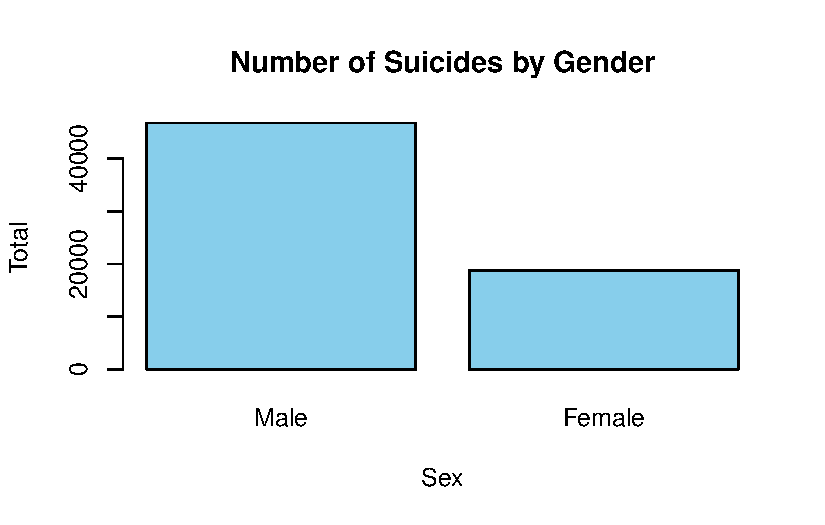
\includegraphics{analysis_files/figure-pdf/unnamed-chunk-2-1.pdf}

}

\end{figure}

\begin{Shaded}
\begin{Highlighting}[]
\NormalTok{b1 }\OtherTok{\textless{}{-}} \FunctionTok{filter}\NormalTok{(data,Sex}\SpecialCharTok{==}\StringTok{"Male"}\NormalTok{,}\StringTok{\textasciigrave{}}\AttributeTok{Age group}\StringTok{\textasciigrave{}}\SpecialCharTok{==}\StringTok{"Total"}\NormalTok{)}
\NormalTok{b2 }\OtherTok{\textless{}{-}} \FunctionTok{filter}\NormalTok{(data,Sex}\SpecialCharTok{==}\StringTok{"Female"}\NormalTok{,}\StringTok{\textasciigrave{}}\AttributeTok{Age group}\StringTok{\textasciigrave{}}\SpecialCharTok{==}\StringTok{"Total"}\NormalTok{)}

\NormalTok{slices }\OtherTok{\textless{}{-}} \FunctionTok{c}\NormalTok{(}\FunctionTok{sum}\NormalTok{(}\FunctionTok{as.numeric}\NormalTok{(b1}\SpecialCharTok{$}\NormalTok{Total)),}\FunctionTok{sum}\NormalTok{(}\FunctionTok{as.numeric}\NormalTok{(b2}\SpecialCharTok{$}\NormalTok{Total)))}

\NormalTok{lbls }\OtherTok{\textless{}{-}} \FunctionTok{c}\NormalTok{(}\StringTok{"Male"}\NormalTok{,}\StringTok{"Female"}\NormalTok{)}
\NormalTok{pct }\OtherTok{\textless{}{-}} \FunctionTok{round}\NormalTok{(slices}\SpecialCharTok{/}\FunctionTok{sum}\NormalTok{(slices)}\SpecialCharTok{*}\DecValTok{100}\NormalTok{)}
\NormalTok{lbls }\OtherTok{\textless{}{-}} \FunctionTok{paste}\NormalTok{(lbls, pct)}
\CommentTok{\# add percents to labels}
\NormalTok{lbls }\OtherTok{\textless{}{-}} \FunctionTok{paste}\NormalTok{(lbls,}\StringTok{"\%"}\NormalTok{,}\AttributeTok{sep=}\StringTok{""}\NormalTok{) }\CommentTok{\# ad \% to labels}
\end{Highlighting}
\end{Shaded}

\begin{Shaded}
\begin{Highlighting}[]
\FunctionTok{pie}\NormalTok{(slices,}\AttributeTok{labels =}\NormalTok{ lbls, }\AttributeTok{col=}\FunctionTok{rainbow}\NormalTok{(}\FunctionTok{length}\NormalTok{(lbls)),}
   \AttributeTok{main=}\StringTok{"Pie Chart of Gender"}\NormalTok{)}
\end{Highlighting}
\end{Shaded}

\begin{figure}[H]

{\centering 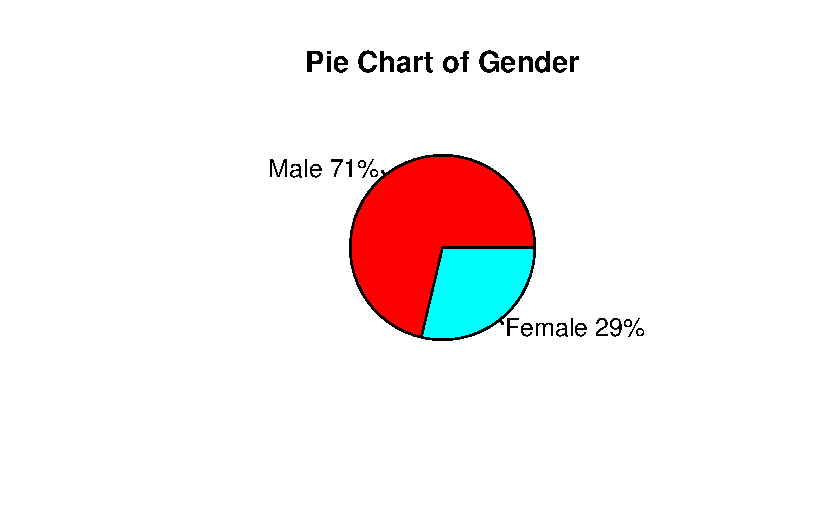
\includegraphics{analysis_files/figure-pdf/unnamed-chunk-4-1.pdf}

}

\end{figure}

-From this graph, we can observe that \textbf{men are more prone to
suicide compared to women}.

\hypertarget{suicides-by-age-groups}{%
\subsection{\texorpdfstring{\textbf{Suicides by Age
Groups}}{Suicides by Age Groups}}\label{suicides-by-age-groups}}

We used the bar plot method to compare suicides by age groups regardless
of gender and reason. You can find the graph and the code we used below.

\begin{Shaded}
\begin{Highlighting}[]
\NormalTok{filtered\_data\_1 }\OtherTok{\textless{}{-}} \FunctionTok{filter}\NormalTok{(data,}\StringTok{\textasciigrave{}}\AttributeTok{Age group}\StringTok{\textasciigrave{}}\SpecialCharTok{==}\StringTok{"\textless{}15"}\NormalTok{, Sex }\SpecialCharTok{==} \StringTok{"Total"}\NormalTok{)}
\NormalTok{filtered\_data\_2 }\OtherTok{\textless{}{-}} \FunctionTok{filter}\NormalTok{(data,}\StringTok{\textasciigrave{}}\AttributeTok{Age group}\StringTok{\textasciigrave{}}\SpecialCharTok{==}\StringTok{"15{-}19"}\NormalTok{, Sex }\SpecialCharTok{==} \StringTok{"Total"}\NormalTok{)}
\NormalTok{filtered\_data\_3 }\OtherTok{\textless{}{-}} \FunctionTok{filter}\NormalTok{(data,}\StringTok{\textasciigrave{}}\AttributeTok{Age group}\StringTok{\textasciigrave{}}\SpecialCharTok{==}\StringTok{"20{-}24"}\NormalTok{, Sex }\SpecialCharTok{==} \StringTok{"Total"}\NormalTok{)}
\NormalTok{filtered\_data\_4 }\OtherTok{\textless{}{-}} \FunctionTok{filter}\NormalTok{(data,}\StringTok{\textasciigrave{}}\AttributeTok{Age group}\StringTok{\textasciigrave{}}\SpecialCharTok{==}\StringTok{"25{-}29"}\NormalTok{, Sex }\SpecialCharTok{==} \StringTok{"Total"}\NormalTok{)}
\NormalTok{filtered\_data\_5 }\OtherTok{\textless{}{-}} \FunctionTok{filter}\NormalTok{(data,}\StringTok{\textasciigrave{}}\AttributeTok{Age group}\StringTok{\textasciigrave{}}\SpecialCharTok{==}\StringTok{"30{-}34"}\NormalTok{, Sex }\SpecialCharTok{==} \StringTok{"Total"}\NormalTok{)}
\NormalTok{filtered\_data\_6 }\OtherTok{\textless{}{-}} \FunctionTok{filter}\NormalTok{(data,}\StringTok{\textasciigrave{}}\AttributeTok{Age group}\StringTok{\textasciigrave{}}\SpecialCharTok{==}\StringTok{"35{-}39"}\NormalTok{, Sex }\SpecialCharTok{==} \StringTok{"Total"}\NormalTok{)}
\NormalTok{filtered\_data\_7 }\OtherTok{\textless{}{-}} \FunctionTok{filter}\NormalTok{(data,}\StringTok{\textasciigrave{}}\AttributeTok{Age group}\StringTok{\textasciigrave{}}\SpecialCharTok{==}\StringTok{"40{-}44"}\NormalTok{, Sex }\SpecialCharTok{==} \StringTok{"Total"}\NormalTok{)}
\NormalTok{filtered\_data\_8 }\OtherTok{\textless{}{-}} \FunctionTok{filter}\NormalTok{(data,}\StringTok{\textasciigrave{}}\AttributeTok{Age group}\StringTok{\textasciigrave{}}\SpecialCharTok{==}\StringTok{"45{-}49"}\NormalTok{, Sex }\SpecialCharTok{==} \StringTok{"Total"}\NormalTok{)}
\NormalTok{filtered\_data\_9 }\OtherTok{\textless{}{-}} \FunctionTok{filter}\NormalTok{(data,}\StringTok{\textasciigrave{}}\AttributeTok{Age group}\StringTok{\textasciigrave{}}\SpecialCharTok{==}\StringTok{"50{-}54"}\NormalTok{, Sex }\SpecialCharTok{==} \StringTok{"Total"}\NormalTok{)}
\NormalTok{filtered\_data\_10 }\OtherTok{\textless{}{-}} \FunctionTok{filter}\NormalTok{(data,}\StringTok{\textasciigrave{}}\AttributeTok{Age group}\StringTok{\textasciigrave{}}\SpecialCharTok{==}\StringTok{"55{-}59"}\NormalTok{, Sex }\SpecialCharTok{==} \StringTok{"Total"}\NormalTok{)}
\NormalTok{filtered\_data\_11 }\OtherTok{\textless{}{-}} \FunctionTok{filter}\NormalTok{(data,}\StringTok{\textasciigrave{}}\AttributeTok{Age group}\StringTok{\textasciigrave{}}\SpecialCharTok{==}\StringTok{"60{-}64"}\NormalTok{, Sex }\SpecialCharTok{==} \StringTok{"Total"}\NormalTok{)}
\NormalTok{filtered\_data\_12 }\OtherTok{\textless{}{-}} \FunctionTok{filter}\NormalTok{(data,}\StringTok{\textasciigrave{}}\AttributeTok{Age group}\StringTok{\textasciigrave{}}\SpecialCharTok{==}\StringTok{"65{-}69"}\NormalTok{, Sex }\SpecialCharTok{==} \StringTok{"Total"}\NormalTok{)}
\NormalTok{filtered\_data\_13 }\OtherTok{\textless{}{-}} \FunctionTok{filter}\NormalTok{(data,}\StringTok{\textasciigrave{}}\AttributeTok{Age group}\StringTok{\textasciigrave{}}\SpecialCharTok{==}\StringTok{"75 +"}\NormalTok{, Sex }\SpecialCharTok{==} \StringTok{"Total"}\NormalTok{)}
\NormalTok{age1 }\OtherTok{=} \FunctionTok{sum}\NormalTok{(}\FunctionTok{as.numeric}\NormalTok{(filtered\_data\_1}\SpecialCharTok{$}\NormalTok{Total))}
\NormalTok{age2 }\OtherTok{=} \FunctionTok{sum}\NormalTok{(}\FunctionTok{as.numeric}\NormalTok{(filtered\_data\_2}\SpecialCharTok{$}\NormalTok{Total))}
\NormalTok{age3 }\OtherTok{=} \FunctionTok{sum}\NormalTok{(}\FunctionTok{as.numeric}\NormalTok{(filtered\_data\_3}\SpecialCharTok{$}\NormalTok{Total))}
\NormalTok{age4 }\OtherTok{=} \FunctionTok{sum}\NormalTok{(}\FunctionTok{as.numeric}\NormalTok{(filtered\_data\_4}\SpecialCharTok{$}\NormalTok{Total))}
\NormalTok{age5 }\OtherTok{=} \FunctionTok{sum}\NormalTok{(}\FunctionTok{as.numeric}\NormalTok{(filtered\_data\_5}\SpecialCharTok{$}\NormalTok{Total))}
\NormalTok{age6 }\OtherTok{=} \FunctionTok{sum}\NormalTok{(}\FunctionTok{as.numeric}\NormalTok{(filtered\_data\_6}\SpecialCharTok{$}\NormalTok{Total))}
\NormalTok{age7 }\OtherTok{=} \FunctionTok{sum}\NormalTok{(}\FunctionTok{as.numeric}\NormalTok{(filtered\_data\_7}\SpecialCharTok{$}\NormalTok{Total))}
\NormalTok{age8 }\OtherTok{=} \FunctionTok{sum}\NormalTok{(}\FunctionTok{as.numeric}\NormalTok{(filtered\_data\_8}\SpecialCharTok{$}\NormalTok{Total))}
\NormalTok{age9 }\OtherTok{=} \FunctionTok{sum}\NormalTok{(}\FunctionTok{as.numeric}\NormalTok{(filtered\_data\_9}\SpecialCharTok{$}\NormalTok{Total))}
\NormalTok{age10 }\OtherTok{=} \FunctionTok{sum}\NormalTok{(}\FunctionTok{as.numeric}\NormalTok{(filtered\_data\_10}\SpecialCharTok{$}\NormalTok{Total))}
\NormalTok{age11 }\OtherTok{=} \FunctionTok{sum}\NormalTok{(}\FunctionTok{as.numeric}\NormalTok{(filtered\_data\_11}\SpecialCharTok{$}\NormalTok{Total))}
\NormalTok{age12 }\OtherTok{=} \FunctionTok{sum}\NormalTok{(}\FunctionTok{as.numeric}\NormalTok{(filtered\_data\_12}\SpecialCharTok{$}\NormalTok{Total))}
\NormalTok{age13 }\OtherTok{=} \FunctionTok{sum}\NormalTok{(}\FunctionTok{as.numeric}\NormalTok{(filtered\_data\_13}\SpecialCharTok{$}\NormalTok{Total))}
\NormalTok{data2 }\OtherTok{=} \FunctionTok{c}\NormalTok{(age1,age2,age3,age4,age5,age6,age7,age8,age9,age10,age11,age12,age13)}
\FunctionTok{barplot}\NormalTok{(data2, }\AttributeTok{names.arg =} \FunctionTok{c}\NormalTok{(}\StringTok{"\textless{}15"}\NormalTok{,}\StringTok{"15{-}19"}\NormalTok{,}\StringTok{"20{-}24"}\NormalTok{,}\StringTok{"25{-}29"}\NormalTok{,}\StringTok{"30{-}34"}\NormalTok{,}\StringTok{"35{-}39"}\NormalTok{,}\StringTok{"40{-}44"}\NormalTok{,}\StringTok{"45{-}49"}\NormalTok{,}\StringTok{"50{-}54"}\NormalTok{,}\StringTok{"55{-}59"}\NormalTok{,}\StringTok{"60{-}64"}\NormalTok{,}\StringTok{"65{-}69"}\NormalTok{,}\StringTok{"75 +"}\NormalTok{), }\AttributeTok{col =} \StringTok{"red"}\NormalTok{, }\AttributeTok{main =} \StringTok{"Number of Suicides by Age Group"}\NormalTok{, }\AttributeTok{xlab =} \StringTok{"Age Group"}\NormalTok{, }\AttributeTok{ylab =} \StringTok{"Total"}\NormalTok{)}
\end{Highlighting}
\end{Shaded}

\begin{figure}[H]

{\centering 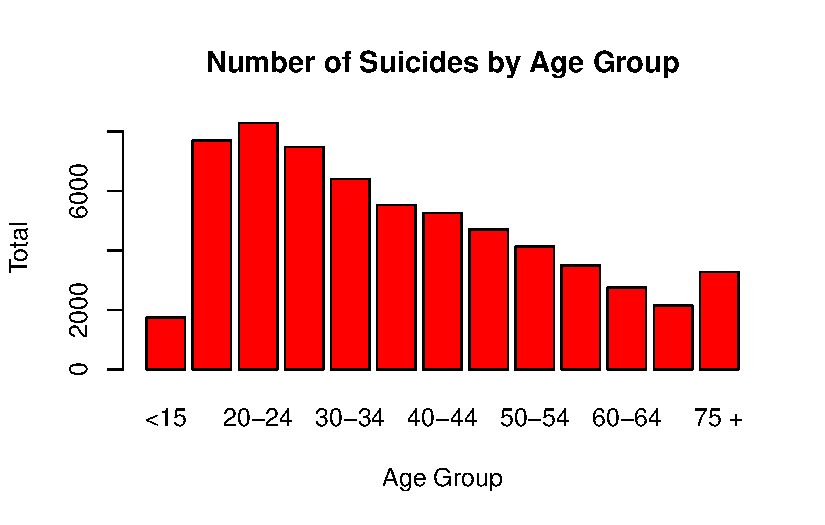
\includegraphics{analysis_files/figure-pdf/unnamed-chunk-5-1.pdf}

}

\end{figure}

When looking at this graph, we observe that \textbf{suicides are most
common among young adults} aged 20-24. We can say that as age progresses
beyond 25, suicide rates tend to decrease. Another interesting result is
that the age groups with the \textbf{lowest suicide rates are children
and the elderly.}

\hypertarget{suicides-by-year}{%
\subsection{\texorpdfstring{\textbf{Suicides by
Year}}{Suicides by Year}}\label{suicides-by-year}}

\begin{Shaded}
\begin{Highlighting}[]
\NormalTok{ffiltered\_data\_1 }\OtherTok{\textless{}{-}} \FunctionTok{filter}\NormalTok{(data,Year}\SpecialCharTok{==}\StringTok{"2002"}\NormalTok{,}\StringTok{\textasciigrave{}}\AttributeTok{Age group}\StringTok{\textasciigrave{}}\SpecialCharTok{==}\StringTok{"Total"}\NormalTok{, Sex }\SpecialCharTok{==} \StringTok{"Total"}\NormalTok{)}
\NormalTok{ffiltered\_data\_2 }\OtherTok{\textless{}{-}} \FunctionTok{filter}\NormalTok{(data,Year}\SpecialCharTok{==}\StringTok{"2003"}\NormalTok{,}\StringTok{\textasciigrave{}}\AttributeTok{Age group}\StringTok{\textasciigrave{}}\SpecialCharTok{==}\StringTok{"Total"}\NormalTok{, Sex }\SpecialCharTok{==} \StringTok{"Total"}\NormalTok{)}
\NormalTok{ffiltered\_data\_3 }\OtherTok{\textless{}{-}} \FunctionTok{filter}\NormalTok{(data,Year}\SpecialCharTok{==}\StringTok{"2004"}\NormalTok{,}\StringTok{\textasciigrave{}}\AttributeTok{Age group}\StringTok{\textasciigrave{}}\SpecialCharTok{==}\StringTok{"Total"}\NormalTok{, Sex }\SpecialCharTok{==} \StringTok{"Total"}\NormalTok{)}
\NormalTok{ffiltered\_data\_4 }\OtherTok{\textless{}{-}} \FunctionTok{filter}\NormalTok{(data,Year}\SpecialCharTok{==}\StringTok{"2005"}\NormalTok{,}\StringTok{\textasciigrave{}}\AttributeTok{Age group}\StringTok{\textasciigrave{}}\SpecialCharTok{==}\StringTok{"Total"}\NormalTok{, Sex }\SpecialCharTok{==} \StringTok{"Total"}\NormalTok{)}
\NormalTok{ffiltered\_data\_5 }\OtherTok{\textless{}{-}} \FunctionTok{filter}\NormalTok{(data,Year}\SpecialCharTok{==}\StringTok{"2006"}\NormalTok{,}\StringTok{\textasciigrave{}}\AttributeTok{Age group}\StringTok{\textasciigrave{}}\SpecialCharTok{==}\StringTok{"Total"}\NormalTok{, Sex }\SpecialCharTok{==} \StringTok{"Total"}\NormalTok{)}
\NormalTok{ffiltered\_data\_6 }\OtherTok{\textless{}{-}} \FunctionTok{filter}\NormalTok{(data,Year}\SpecialCharTok{==}\StringTok{"2007"}\NormalTok{,}\StringTok{\textasciigrave{}}\AttributeTok{Age group}\StringTok{\textasciigrave{}}\SpecialCharTok{==}\StringTok{"Total"}\NormalTok{, Sex }\SpecialCharTok{==} \StringTok{"Total"}\NormalTok{)}
\NormalTok{ffiltered\_data\_7 }\OtherTok{\textless{}{-}} \FunctionTok{filter}\NormalTok{(data,Year}\SpecialCharTok{==}\StringTok{"2008"}\NormalTok{,}\StringTok{\textasciigrave{}}\AttributeTok{Age group}\StringTok{\textasciigrave{}}\SpecialCharTok{==}\StringTok{"Total"}\NormalTok{, Sex }\SpecialCharTok{==} \StringTok{"Total"}\NormalTok{)}
\NormalTok{ffiltered\_data\_8 }\OtherTok{\textless{}{-}} \FunctionTok{filter}\NormalTok{(data,Year}\SpecialCharTok{==}\StringTok{"2009"}\NormalTok{,}\StringTok{\textasciigrave{}}\AttributeTok{Age group}\StringTok{\textasciigrave{}}\SpecialCharTok{==}\StringTok{"Total"}\NormalTok{, Sex }\SpecialCharTok{==} \StringTok{"Total"}\NormalTok{)}
\NormalTok{ffiltered\_data\_9 }\OtherTok{\textless{}{-}} \FunctionTok{filter}\NormalTok{(data,Year}\SpecialCharTok{==}\StringTok{"2010"}\NormalTok{,}\StringTok{\textasciigrave{}}\AttributeTok{Age group}\StringTok{\textasciigrave{}}\SpecialCharTok{==}\StringTok{"Total"}\NormalTok{, Sex }\SpecialCharTok{==} \StringTok{"Total"}\NormalTok{)}
\NormalTok{ffiltered\_data\_10 }\OtherTok{\textless{}{-}} \FunctionTok{filter}\NormalTok{(data,Year}\SpecialCharTok{==}\StringTok{"2011"}\NormalTok{,}\StringTok{\textasciigrave{}}\AttributeTok{Age group}\StringTok{\textasciigrave{}}\SpecialCharTok{==}\StringTok{"Total"}\NormalTok{, Sex }\SpecialCharTok{==} \StringTok{"Total"}\NormalTok{)}
\NormalTok{ffiltered\_data\_11 }\OtherTok{\textless{}{-}} \FunctionTok{filter}\NormalTok{(data,Year}\SpecialCharTok{==}\StringTok{"2012"}\NormalTok{,}\StringTok{\textasciigrave{}}\AttributeTok{Age group}\StringTok{\textasciigrave{}}\SpecialCharTok{==}\StringTok{"Total"}\NormalTok{, Sex }\SpecialCharTok{==} \StringTok{"Total"}\NormalTok{)}
\NormalTok{ffiltered\_data\_12 }\OtherTok{\textless{}{-}} \FunctionTok{filter}\NormalTok{(data,Year}\SpecialCharTok{==}\StringTok{"2013"}\NormalTok{,}\StringTok{\textasciigrave{}}\AttributeTok{Age group}\StringTok{\textasciigrave{}}\SpecialCharTok{==}\StringTok{"Total"}\NormalTok{, Sex }\SpecialCharTok{==} \StringTok{"Total"}\NormalTok{)}
\NormalTok{ffiltered\_data\_13 }\OtherTok{\textless{}{-}} \FunctionTok{filter}\NormalTok{(data,Year}\SpecialCharTok{==}\StringTok{"2014"}\NormalTok{,}\StringTok{\textasciigrave{}}\AttributeTok{Age group}\StringTok{\textasciigrave{}}\SpecialCharTok{==}\StringTok{"Total"}\NormalTok{, Sex }\SpecialCharTok{==} \StringTok{"Total"}\NormalTok{)}
\NormalTok{ffiltered\_data\_14 }\OtherTok{\textless{}{-}} \FunctionTok{filter}\NormalTok{(data,Year}\SpecialCharTok{==}\StringTok{"2015"}\NormalTok{,}\StringTok{\textasciigrave{}}\AttributeTok{Age group}\StringTok{\textasciigrave{}}\SpecialCharTok{==}\StringTok{"Total"}\NormalTok{, Sex }\SpecialCharTok{==} \StringTok{"Total"}\NormalTok{)}
\NormalTok{ffiltered\_data\_15 }\OtherTok{\textless{}{-}} \FunctionTok{filter}\NormalTok{(data,Year}\SpecialCharTok{==}\StringTok{"2016"}\NormalTok{,}\StringTok{\textasciigrave{}}\AttributeTok{Age group}\StringTok{\textasciigrave{}}\SpecialCharTok{==}\StringTok{"Total"}\NormalTok{, Sex }\SpecialCharTok{==} \StringTok{"Total"}\NormalTok{)}
\NormalTok{ffiltered\_data\_16 }\OtherTok{\textless{}{-}} \FunctionTok{filter}\NormalTok{(data,Year}\SpecialCharTok{==}\StringTok{"2017"}\NormalTok{,}\StringTok{\textasciigrave{}}\AttributeTok{Age group}\StringTok{\textasciigrave{}}\SpecialCharTok{==}\StringTok{"Total"}\NormalTok{, Sex }\SpecialCharTok{==} \StringTok{"Total"}\NormalTok{)}
\NormalTok{ffiltered\_data\_17 }\OtherTok{\textless{}{-}} \FunctionTok{filter}\NormalTok{(data,Year}\SpecialCharTok{==}\StringTok{"2018"}\NormalTok{,}\StringTok{\textasciigrave{}}\AttributeTok{Age group}\StringTok{\textasciigrave{}}\SpecialCharTok{==}\StringTok{"Total"}\NormalTok{, Sex }\SpecialCharTok{==} \StringTok{"Total"}\NormalTok{)}
\NormalTok{ffiltered\_data\_18 }\OtherTok{\textless{}{-}} \FunctionTok{filter}\NormalTok{(data,Year}\SpecialCharTok{==}\StringTok{"2019"}\NormalTok{,}\StringTok{\textasciigrave{}}\AttributeTok{Age group}\StringTok{\textasciigrave{}}\SpecialCharTok{==}\StringTok{"Total"}\NormalTok{, Sex }\SpecialCharTok{==} \StringTok{"Total"}\NormalTok{)}
\NormalTok{ffiltered\_data\_19 }\OtherTok{\textless{}{-}} \FunctionTok{filter}\NormalTok{(data,Year}\SpecialCharTok{==}\StringTok{"2020"}\NormalTok{,}\StringTok{\textasciigrave{}}\AttributeTok{Age group}\StringTok{\textasciigrave{}}\SpecialCharTok{==}\StringTok{"Total"}\NormalTok{, Sex }\SpecialCharTok{==} \StringTok{"Total"}\NormalTok{)}
\NormalTok{ffiltered\_data\_20 }\OtherTok{\textless{}{-}} \FunctionTok{filter}\NormalTok{(data,Year}\SpecialCharTok{==}\StringTok{"2021"}\NormalTok{,}\StringTok{\textasciigrave{}}\AttributeTok{Age group}\StringTok{\textasciigrave{}}\SpecialCharTok{==}\StringTok{"Total"}\NormalTok{, Sex }\SpecialCharTok{==} \StringTok{"Total"}\NormalTok{)}
\NormalTok{ffiltered\_data\_21 }\OtherTok{\textless{}{-}} \FunctionTok{filter}\NormalTok{(data,Year}\SpecialCharTok{==}\StringTok{"2022"}\NormalTok{,}\StringTok{\textasciigrave{}}\AttributeTok{Age group}\StringTok{\textasciigrave{}}\SpecialCharTok{==}\StringTok{"Total"}\NormalTok{, Sex }\SpecialCharTok{==} \StringTok{"Total"}\NormalTok{)}

\NormalTok{year1 }\OtherTok{=} \FunctionTok{sum}\NormalTok{(}\FunctionTok{as.numeric}\NormalTok{(ffiltered\_data\_1}\SpecialCharTok{$}\NormalTok{Total))}
\NormalTok{year2 }\OtherTok{=} \FunctionTok{sum}\NormalTok{(}\FunctionTok{as.numeric}\NormalTok{(ffiltered\_data\_2}\SpecialCharTok{$}\NormalTok{Total))}
\NormalTok{year3 }\OtherTok{=} \FunctionTok{sum}\NormalTok{(}\FunctionTok{as.numeric}\NormalTok{(ffiltered\_data\_3}\SpecialCharTok{$}\NormalTok{Total))}
\NormalTok{year4 }\OtherTok{=} \FunctionTok{sum}\NormalTok{(}\FunctionTok{as.numeric}\NormalTok{(ffiltered\_data\_4}\SpecialCharTok{$}\NormalTok{Total))}
\NormalTok{year5 }\OtherTok{=} \FunctionTok{sum}\NormalTok{(}\FunctionTok{as.numeric}\NormalTok{(ffiltered\_data\_5}\SpecialCharTok{$}\NormalTok{Total))}
\NormalTok{year6 }\OtherTok{=} \FunctionTok{sum}\NormalTok{(}\FunctionTok{as.numeric}\NormalTok{(ffiltered\_data\_6}\SpecialCharTok{$}\NormalTok{Total))}
\NormalTok{year7 }\OtherTok{=} \FunctionTok{sum}\NormalTok{(}\FunctionTok{as.numeric}\NormalTok{(ffiltered\_data\_7}\SpecialCharTok{$}\NormalTok{Total))}
\NormalTok{year8 }\OtherTok{=} \FunctionTok{sum}\NormalTok{(}\FunctionTok{as.numeric}\NormalTok{(ffiltered\_data\_8}\SpecialCharTok{$}\NormalTok{Total))}
\NormalTok{year9 }\OtherTok{=} \FunctionTok{sum}\NormalTok{(}\FunctionTok{as.numeric}\NormalTok{(ffiltered\_data\_9}\SpecialCharTok{$}\NormalTok{Total))}
\NormalTok{year10 }\OtherTok{=} \FunctionTok{sum}\NormalTok{(}\FunctionTok{as.numeric}\NormalTok{(ffiltered\_data\_10}\SpecialCharTok{$}\NormalTok{Total))}
\NormalTok{year11 }\OtherTok{=} \FunctionTok{sum}\NormalTok{(}\FunctionTok{as.numeric}\NormalTok{(ffiltered\_data\_11}\SpecialCharTok{$}\NormalTok{Total))}
\NormalTok{year12 }\OtherTok{=} \FunctionTok{sum}\NormalTok{(}\FunctionTok{as.numeric}\NormalTok{(ffiltered\_data\_12}\SpecialCharTok{$}\NormalTok{Total))}
\NormalTok{year13 }\OtherTok{=} \FunctionTok{sum}\NormalTok{(}\FunctionTok{as.numeric}\NormalTok{(ffiltered\_data\_13}\SpecialCharTok{$}\NormalTok{Total))}
\NormalTok{year14 }\OtherTok{=} \FunctionTok{sum}\NormalTok{(}\FunctionTok{as.numeric}\NormalTok{(ffiltered\_data\_14}\SpecialCharTok{$}\NormalTok{Total))}
\NormalTok{year15 }\OtherTok{=} \FunctionTok{sum}\NormalTok{(}\FunctionTok{as.numeric}\NormalTok{(ffiltered\_data\_15}\SpecialCharTok{$}\NormalTok{Total))}
\NormalTok{year16 }\OtherTok{=} \FunctionTok{sum}\NormalTok{(}\FunctionTok{as.numeric}\NormalTok{(ffiltered\_data\_16}\SpecialCharTok{$}\NormalTok{Total))}
\NormalTok{year17 }\OtherTok{=} \FunctionTok{sum}\NormalTok{(}\FunctionTok{as.numeric}\NormalTok{(ffiltered\_data\_17}\SpecialCharTok{$}\NormalTok{Total))}
\NormalTok{year18 }\OtherTok{=} \FunctionTok{sum}\NormalTok{(}\FunctionTok{as.numeric}\NormalTok{(ffiltered\_data\_18}\SpecialCharTok{$}\NormalTok{Total))}
\NormalTok{year19 }\OtherTok{=} \FunctionTok{sum}\NormalTok{(}\FunctionTok{as.numeric}\NormalTok{(ffiltered\_data\_19}\SpecialCharTok{$}\NormalTok{Total))}
\NormalTok{year20 }\OtherTok{=} \FunctionTok{sum}\NormalTok{(}\FunctionTok{as.numeric}\NormalTok{(ffiltered\_data\_20}\SpecialCharTok{$}\NormalTok{Total))}
\NormalTok{year21 }\OtherTok{=} \FunctionTok{sum}\NormalTok{(}\FunctionTok{as.numeric}\NormalTok{(ffiltered\_data\_21}\SpecialCharTok{$}\NormalTok{Total))}
\end{Highlighting}
\end{Shaded}

\begin{Shaded}
\begin{Highlighting}[]
\NormalTok{data3 }\OtherTok{=} \FunctionTok{c}\NormalTok{(year1,year2,year3,year4,year5,year6,year7,year8,year9,year10,year11,year12,year13,year14,year15,year16,year17,year18,year19,year20,year21)}
\FunctionTok{barplot}\NormalTok{(data3, }\AttributeTok{names.arg =} \FunctionTok{c}\NormalTok{(}\StringTok{"2002"}\NormalTok{,}\StringTok{"2003"}\NormalTok{,}\StringTok{"2004"}\NormalTok{,}\StringTok{"2005"}\NormalTok{,}\StringTok{"2006"}\NormalTok{,}\StringTok{"2007"}\NormalTok{,}\StringTok{"2008"}\NormalTok{,}\StringTok{"2009"}\NormalTok{,}\StringTok{"2010"}\NormalTok{,}\StringTok{"2011"}\NormalTok{,}\StringTok{"2012"}\NormalTok{,}\StringTok{"2013"}\NormalTok{,}\StringTok{"2014"}\NormalTok{,}\StringTok{"2015"}\NormalTok{,}\StringTok{"2016"}\NormalTok{,}\StringTok{"2017"}\NormalTok{,}\StringTok{"2018"}\NormalTok{,}\StringTok{"2019"}\NormalTok{,}\StringTok{"2020"}\NormalTok{,}\StringTok{"2021"}\NormalTok{,}\StringTok{"2022"}\NormalTok{), }\AttributeTok{col =} \StringTok{"yellow"}\NormalTok{, }\AttributeTok{main =} \StringTok{"Number of Suicides by Year"}\NormalTok{, }\AttributeTok{xlab =} \StringTok{"Year"}\NormalTok{, }\AttributeTok{ylab =} \StringTok{"Total"}\NormalTok{)}
\end{Highlighting}
\end{Shaded}

\begin{figure}[H]

{\centering 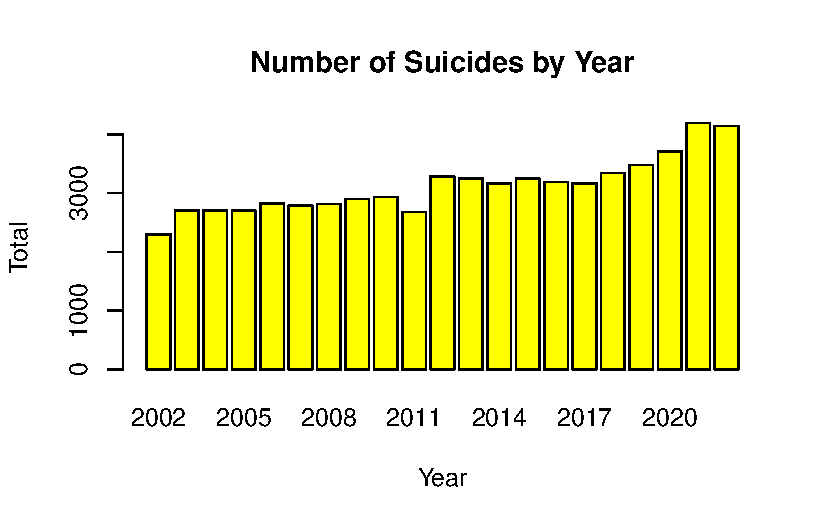
\includegraphics{analysis_files/figure-pdf/unnamed-chunk-7-1.pdf}

}

\end{figure}

\hypertarget{suicides-by-reason}{%
\subsection{\texorpdfstring{\textbf{Suicides by
Reason}}{Suicides by Reason}}\label{suicides-by-reason}}

\begin{Shaded}
\begin{Highlighting}[]
\NormalTok{fffiltered\_data\_1 }\OtherTok{\textless{}{-}} \FunctionTok{filter}\NormalTok{(data,}\StringTok{\textasciigrave{}}\AttributeTok{Age group}\StringTok{\textasciigrave{}}\SpecialCharTok{==}\StringTok{"Total"}\NormalTok{, Sex }\SpecialCharTok{==} \StringTok{"Total"}\NormalTok{)}
\NormalTok{cause1 }\OtherTok{=} \FunctionTok{sum}\NormalTok{(}\FunctionTok{as.numeric}\NormalTok{(fffiltered\_data\_1}\SpecialCharTok{$}\NormalTok{Illness))}
\NormalTok{cause2 }\OtherTok{=} \FunctionTok{sum}\NormalTok{(}\FunctionTok{as.numeric}\NormalTok{(fffiltered\_data\_1}\SpecialCharTok{$}\StringTok{\textasciigrave{}}\AttributeTok{Family incompatibility}\StringTok{\textasciigrave{}}\NormalTok{))}
\NormalTok{cause3 }\OtherTok{=} \FunctionTok{sum}\NormalTok{(}\FunctionTok{as.numeric}\NormalTok{(fffiltered\_data\_1}\SpecialCharTok{$}\StringTok{\textasciigrave{}}\AttributeTok{Economic problems}\StringTok{\textasciigrave{}}\NormalTok{))}
\NormalTok{cause4 }\OtherTok{=} \FunctionTok{sum}\NormalTok{(}\FunctionTok{as.numeric}\NormalTok{(fffiltered\_data\_1}\SpecialCharTok{$}\StringTok{\textasciigrave{}}\AttributeTok{Business failure}\StringTok{\textasciigrave{}}\NormalTok{))}
\NormalTok{cause5 }\OtherTok{=} \FunctionTok{sum}\NormalTok{(}\FunctionTok{as.numeric}\NormalTok{(fffiltered\_data\_1}\SpecialCharTok{$}\StringTok{\textasciigrave{}}\AttributeTok{Emotional relationship and not marrying the person wanted}\StringTok{\textasciigrave{}}\NormalTok{))}
\NormalTok{cause6 }\OtherTok{=} \FunctionTok{sum}\NormalTok{(}\FunctionTok{as.numeric}\NormalTok{(fffiltered\_data\_1}\SpecialCharTok{$}\StringTok{\textasciigrave{}}\AttributeTok{Educational failure}\StringTok{\textasciigrave{}}\NormalTok{))}
\NormalTok{cause7 }\OtherTok{=} \FunctionTok{sum}\NormalTok{(}\FunctionTok{as.numeric}\NormalTok{(fffiltered\_data\_1}\SpecialCharTok{$}\NormalTok{Other))}
\NormalTok{unknown }\OtherTok{\textless{}{-}} \FunctionTok{ifelse}\NormalTok{(}\FunctionTok{is.na}\NormalTok{(}\FunctionTok{as.numeric}\NormalTok{(fffiltered\_data\_1}\SpecialCharTok{$}\NormalTok{Unknown)),}\DecValTok{0}\NormalTok{,}\FunctionTok{as.numeric}\NormalTok{(fffiltered\_data\_1}\SpecialCharTok{$}\NormalTok{Unknown))}
\NormalTok{cause8 }\OtherTok{=} \FunctionTok{sum}\NormalTok{(unknown)}
\NormalTok{data4 }\OtherTok{=} \FunctionTok{c}\NormalTok{(cause1,cause2,cause3,cause4,cause5,cause6,cause7,cause8)}
\end{Highlighting}
\end{Shaded}

\begin{Shaded}
\begin{Highlighting}[]
\FunctionTok{barplot}\NormalTok{(data4, }\AttributeTok{names.arg =} \FunctionTok{c}\NormalTok{(}\StringTok{"Illness"}\NormalTok{,}\StringTok{"Family"}\NormalTok{,}\StringTok{"Economy"}\NormalTok{,}\StringTok{"Business"}\NormalTok{,}\StringTok{"Emotional"}\NormalTok{,}\StringTok{"Educational"}\NormalTok{,}\StringTok{"Other"}\NormalTok{,}\StringTok{"Unknown"}\NormalTok{), }\AttributeTok{col =} \StringTok{"brown"}\NormalTok{, }\AttributeTok{main =} \StringTok{"Number of Suicides by Reason"}\NormalTok{, }\AttributeTok{xlab =} \StringTok{"Suicide Reason"}\NormalTok{, }\AttributeTok{ylab =} \StringTok{"Total"}\NormalTok{,}\AttributeTok{cex.names=}\FloatTok{0.72}\NormalTok{)}
\end{Highlighting}
\end{Shaded}

\begin{figure}[H]

{\centering 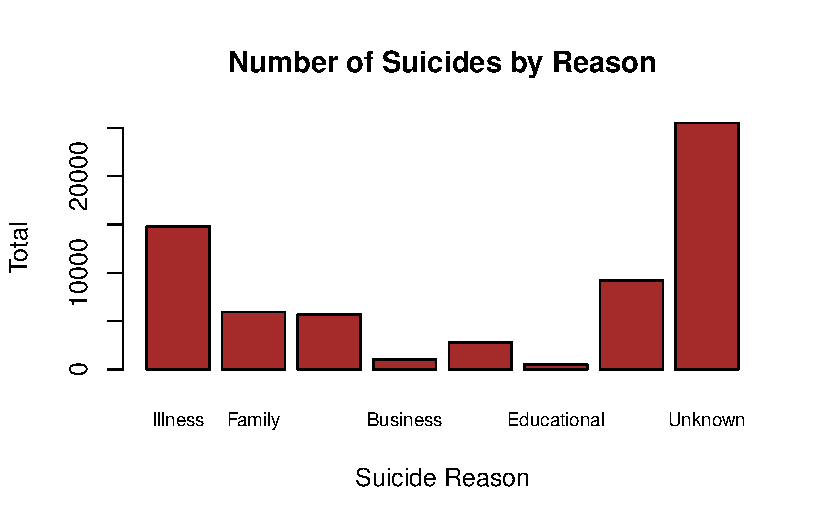
\includegraphics{analysis_files/figure-pdf/unnamed-chunk-9-1.pdf}

}

\end{figure}

\begin{Shaded}
\begin{Highlighting}[]
\CommentTok{\# Keep only 3 names}
\NormalTok{  a }\OtherTok{=} \FunctionTok{filter}\NormalTok{(data,Year }\SpecialCharTok{!=} \StringTok{"2002"}\NormalTok{,Year}\SpecialCharTok{!=}\StringTok{"2003"}\NormalTok{,}\StringTok{\textasciigrave{}}\AttributeTok{Age group}\StringTok{\textasciigrave{}}\SpecialCharTok{==}\StringTok{"Total"}\NormalTok{, Sex }\SpecialCharTok{==} \StringTok{"Total"}\NormalTok{)}
\NormalTok{  a1 }\OtherTok{=} \FunctionTok{data.frame}\NormalTok{(}\AttributeTok{Year=}\NormalTok{a}\SpecialCharTok{$}\NormalTok{Year,}\AttributeTok{Total=}\NormalTok{a}\SpecialCharTok{$}\NormalTok{Illness,}\AttributeTok{Cause=}\StringTok{"Illness"}\NormalTok{)}
\NormalTok{  a2 }\OtherTok{=} \FunctionTok{data.frame}\NormalTok{(}\AttributeTok{Year=}\NormalTok{a}\SpecialCharTok{$}\NormalTok{Year,}\AttributeTok{Total=}\NormalTok{a}\SpecialCharTok{$}\StringTok{\textasciigrave{}}\AttributeTok{Family incompatibility}\StringTok{\textasciigrave{}}\NormalTok{,}\AttributeTok{Cause=}\StringTok{"Family"}\NormalTok{)}
\NormalTok{  a3 }\OtherTok{=} \FunctionTok{data.frame}\NormalTok{(}\AttributeTok{Year=}\NormalTok{a}\SpecialCharTok{$}\NormalTok{Year,}\AttributeTok{Total=}\NormalTok{a}\SpecialCharTok{$}\StringTok{\textasciigrave{}}\AttributeTok{Economic problems}\StringTok{\textasciigrave{}}\NormalTok{,}\AttributeTok{Cause=}\StringTok{"Economy"}\NormalTok{)}
\NormalTok{  a4 }\OtherTok{=} \FunctionTok{data.frame}\NormalTok{(}\AttributeTok{Year=}\NormalTok{a}\SpecialCharTok{$}\NormalTok{Year,}\AttributeTok{Total=}\NormalTok{a}\SpecialCharTok{$}\StringTok{\textasciigrave{}}\AttributeTok{Business failure}\StringTok{\textasciigrave{}}\NormalTok{,}\AttributeTok{Cause=}\StringTok{"Business"}\NormalTok{)}
\NormalTok{  a5 }\OtherTok{=} \FunctionTok{data.frame}\NormalTok{(}\AttributeTok{Year=}\NormalTok{a}\SpecialCharTok{$}\NormalTok{Year,}\AttributeTok{Total=}\NormalTok{a}\SpecialCharTok{$}\StringTok{\textasciigrave{}}\AttributeTok{Emotional relationship and not marrying the person wanted}\StringTok{\textasciigrave{}}\NormalTok{,}\AttributeTok{Cause=}\StringTok{"Emotional"}\NormalTok{)}
\NormalTok{  a6 }\OtherTok{=} \FunctionTok{data.frame}\NormalTok{(}\AttributeTok{Year=}\NormalTok{a}\SpecialCharTok{$}\NormalTok{Year,}\AttributeTok{Total=}\NormalTok{a}\SpecialCharTok{$}\StringTok{\textasciigrave{}}\AttributeTok{Educational failure}\StringTok{\textasciigrave{}}\NormalTok{,}\AttributeTok{Cause=}\StringTok{"Education"}\NormalTok{)}
\NormalTok{  a7 }\OtherTok{=} \FunctionTok{data.frame}\NormalTok{(}\AttributeTok{Year=}\NormalTok{a}\SpecialCharTok{$}\NormalTok{Year,}\AttributeTok{Total=}\NormalTok{a}\SpecialCharTok{$}\NormalTok{Other,}\AttributeTok{Cause=}\StringTok{"Other"}\NormalTok{)}
\NormalTok{  a8 }\OtherTok{=} \FunctionTok{data.frame}\NormalTok{(}\AttributeTok{Year=}\NormalTok{a}\SpecialCharTok{$}\NormalTok{Year,}\AttributeTok{Total=}\NormalTok{a}\SpecialCharTok{$}\NormalTok{Unknown,}\AttributeTok{Cause=}\StringTok{"Unknown"}\NormalTok{)}
\NormalTok{  cause }\OtherTok{=} \FunctionTok{rbind}\NormalTok{(a1,a2,a3,a4,a5,a6,a7,a8,}\AttributeTok{deparse.level =} \DecValTok{0}\NormalTok{)}
\end{Highlighting}
\end{Shaded}

\begin{Shaded}
\begin{Highlighting}[]
\NormalTok{graph }\OtherTok{\textless{}{-}}\NormalTok{ cause }\SpecialCharTok{\%\textgreater{}\%} 
    \FunctionTok{filter}\NormalTok{(Cause }\SpecialCharTok{\%in\%} \FunctionTok{c}\NormalTok{(}\StringTok{"Illness"}\NormalTok{,}\StringTok{"Family"}\NormalTok{,}\StringTok{"Economy"}\NormalTok{,}\StringTok{"Business"}\NormalTok{,}\StringTok{"Emotional"}\NormalTok{,}\StringTok{"Education"}\NormalTok{,}\StringTok{"Other"}\NormalTok{,}\StringTok{"Unknown"}\NormalTok{))}
\NormalTok{  b }\OtherTok{=} \FunctionTok{as.numeric}\NormalTok{(cause}\SpecialCharTok{$}\NormalTok{Total)}
\NormalTok{  c }\OtherTok{=} \FunctionTok{ifelse}\NormalTok{(}\FunctionTok{is.na}\NormalTok{(b),}\DecValTok{0}\NormalTok{,b)}
\NormalTok{  graph }\SpecialCharTok{\%\textgreater{}\%}
    \FunctionTok{ggplot}\NormalTok{( }\FunctionTok{aes}\NormalTok{(}\AttributeTok{x=}\NormalTok{Year, }\AttributeTok{y=}\NormalTok{c, }\AttributeTok{group=}\NormalTok{Cause, }\AttributeTok{color=}\NormalTok{Cause)) }\SpecialCharTok{+}
      \FunctionTok{geom\_line}\NormalTok{() }\SpecialCharTok{+}
      \FunctionTok{ylab}\NormalTok{(}\StringTok{"Number of Suicides"}\NormalTok{) }\SpecialCharTok{+}
      \FunctionTok{scale\_y\_log10}\NormalTok{() }\SpecialCharTok{+}
      \FunctionTok{ggtitle}\NormalTok{(}\StringTok{"Number of Suicides by Reasons"}\NormalTok{)}
\end{Highlighting}
\end{Shaded}

\begin{figure}[H]

{\centering 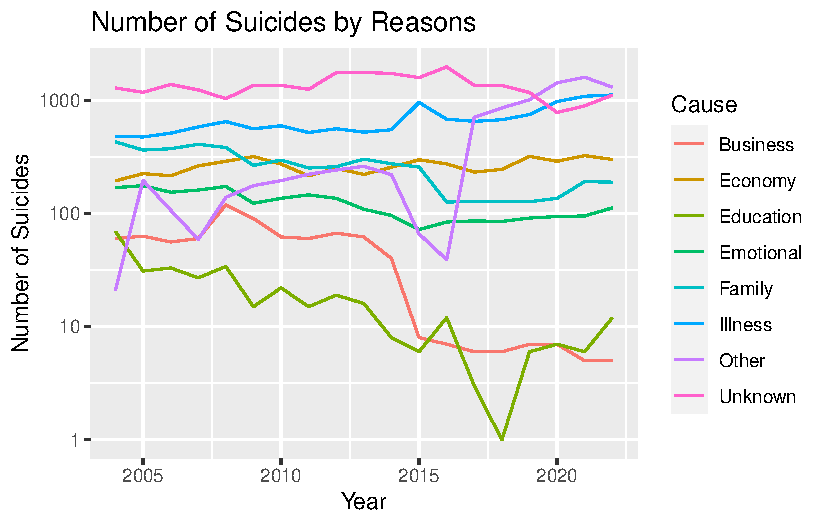
\includegraphics{analysis_files/figure-pdf/unnamed-chunk-11-1.pdf}

}

\end{figure}

\begin{Shaded}
\begin{Highlighting}[]
\CommentTok{\# Pie Chart with Percentages}
\CommentTok{\#| codefold: true}
\CommentTok{\#| output: false}
\NormalTok{slices }\OtherTok{\textless{}{-}} \FunctionTok{c}\NormalTok{(}
  \FunctionTok{sum}\NormalTok{(}\FunctionTok{ifelse}\NormalTok{(}\FunctionTok{is.na}\NormalTok{(}\FunctionTok{as.numeric}\NormalTok{(a}\SpecialCharTok{$}\NormalTok{Illness)),}\DecValTok{0}\NormalTok{,}\FunctionTok{as.numeric}\NormalTok{(a}\SpecialCharTok{$}\NormalTok{Illness))),}
  \FunctionTok{sum}\NormalTok{(}\FunctionTok{ifelse}\NormalTok{(}\FunctionTok{is.na}\NormalTok{(}\FunctionTok{as.numeric}\NormalTok{(a}\SpecialCharTok{$}\StringTok{\textasciigrave{}}\AttributeTok{Family incompatibility}\StringTok{\textasciigrave{}}\NormalTok{)),}\DecValTok{0}\NormalTok{,}\FunctionTok{as.numeric}\NormalTok{(a}\SpecialCharTok{$}\StringTok{\textasciigrave{}}\AttributeTok{Family incompatibility}\StringTok{\textasciigrave{}}\NormalTok{))) ,}
  \FunctionTok{sum}\NormalTok{(}\FunctionTok{ifelse}\NormalTok{(}\FunctionTok{is.na}\NormalTok{(}\FunctionTok{as.numeric}\NormalTok{(a}\SpecialCharTok{$}\StringTok{\textasciigrave{}}\AttributeTok{Economic problems}\StringTok{\textasciigrave{}}\NormalTok{)),}\DecValTok{0}\NormalTok{,}\FunctionTok{as.numeric}\NormalTok{(a}\SpecialCharTok{$}\StringTok{\textasciigrave{}}\AttributeTok{Economic problems}\StringTok{\textasciigrave{}}\NormalTok{))),}
  \FunctionTok{sum}\NormalTok{(}\FunctionTok{ifelse}\NormalTok{(}\FunctionTok{is.na}\NormalTok{(}\FunctionTok{as.numeric}\NormalTok{(a}\SpecialCharTok{$}\StringTok{\textasciigrave{}}\AttributeTok{Business failure}\StringTok{\textasciigrave{}}\NormalTok{)),}\DecValTok{0}\NormalTok{,}\FunctionTok{as.numeric}\NormalTok{(a}\SpecialCharTok{$}\StringTok{\textasciigrave{}}\AttributeTok{Business failure}\StringTok{\textasciigrave{}}\NormalTok{))),}
  \FunctionTok{sum}\NormalTok{(}\FunctionTok{ifelse}\NormalTok{(}\FunctionTok{is.na}\NormalTok{(}\FunctionTok{as.numeric}\NormalTok{(a}\SpecialCharTok{$}\StringTok{\textasciigrave{}}\AttributeTok{Emotional relationship and not marrying the person wanted}\StringTok{\textasciigrave{}}\NormalTok{)),}\DecValTok{0}\NormalTok{,}\FunctionTok{as.numeric}\NormalTok{(a}\SpecialCharTok{$}\StringTok{\textasciigrave{}}\AttributeTok{Emotional relationship and not marrying the person wanted}\StringTok{\textasciigrave{}}\NormalTok{))),}
  \FunctionTok{sum}\NormalTok{(}\FunctionTok{ifelse}\NormalTok{(}\FunctionTok{is.na}\NormalTok{(}\FunctionTok{as.numeric}\NormalTok{(a}\SpecialCharTok{$}\StringTok{\textasciigrave{}}\AttributeTok{Educational failure}\StringTok{\textasciigrave{}}\NormalTok{)),}\DecValTok{0}\NormalTok{,}\FunctionTok{as.numeric}\NormalTok{(a}\SpecialCharTok{$}\StringTok{\textasciigrave{}}\AttributeTok{Educational failure}\StringTok{\textasciigrave{}}\NormalTok{))),}
  \FunctionTok{sum}\NormalTok{(}\FunctionTok{ifelse}\NormalTok{(}\FunctionTok{is.na}\NormalTok{(}\FunctionTok{as.numeric}\NormalTok{(a}\SpecialCharTok{$}\NormalTok{Other)),}\DecValTok{0}\NormalTok{,}\FunctionTok{as.numeric}\NormalTok{(a}\SpecialCharTok{$}\NormalTok{Other))),}\FunctionTok{sum}\NormalTok{(}\FunctionTok{ifelse}\NormalTok{(}\FunctionTok{is.na}\NormalTok{(}\FunctionTok{as.numeric}\NormalTok{(a}\SpecialCharTok{$}\NormalTok{Unknown)),}\DecValTok{0}\NormalTok{,}\FunctionTok{as.numeric}\NormalTok{(a}\SpecialCharTok{$}\NormalTok{Unknown))))}

\NormalTok{lbls }\OtherTok{\textless{}{-}} \FunctionTok{c}\NormalTok{(}\StringTok{"Illness"}\NormalTok{,}\StringTok{"Family"}\NormalTok{,}\StringTok{"Economy"}\NormalTok{,}\StringTok{"Business"}\NormalTok{,}\StringTok{"Emotional"}\NormalTok{,}\StringTok{"Education"}\NormalTok{,}\StringTok{"Other"}\NormalTok{,}\StringTok{"Unknown"}\NormalTok{)}
\NormalTok{pct }\OtherTok{\textless{}{-}} \FunctionTok{round}\NormalTok{(slices}\SpecialCharTok{/}\FunctionTok{sum}\NormalTok{(slices)}\SpecialCharTok{*}\DecValTok{100}\NormalTok{)}
\NormalTok{lbls }\OtherTok{\textless{}{-}} \FunctionTok{paste}\NormalTok{(lbls, pct)}
\CommentTok{\# add percents to labels}
\NormalTok{lbls }\OtherTok{\textless{}{-}} \FunctionTok{paste}\NormalTok{(lbls,}\StringTok{"\%"}\NormalTok{,}\AttributeTok{sep=}\StringTok{""}\NormalTok{) }\CommentTok{\# ad \% to labels}
\end{Highlighting}
\end{Shaded}

\begin{Shaded}
\begin{Highlighting}[]
\FunctionTok{pie}\NormalTok{(slices,}\AttributeTok{labels =}\NormalTok{ lbls, }\AttributeTok{col=}\FunctionTok{rainbow}\NormalTok{(}\FunctionTok{length}\NormalTok{(lbls)),}
   \AttributeTok{main=}\StringTok{"Pie Chart of Suicide Reasons"}\NormalTok{,}\AttributeTok{cex=}\FloatTok{0.8}\NormalTok{)}
\end{Highlighting}
\end{Shaded}

\begin{figure}[H]

{\centering 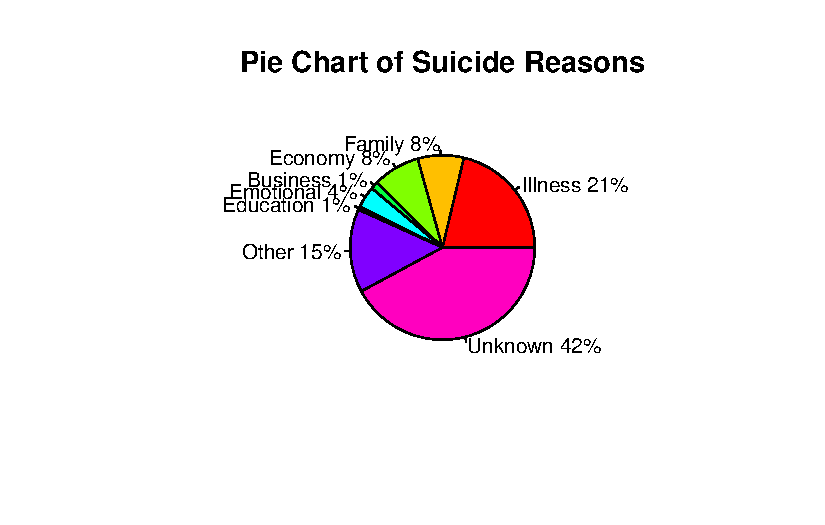
\includegraphics{analysis_files/figure-pdf/unnamed-chunk-13-1.pdf}

}

\end{figure}

\begin{Shaded}
\begin{Highlighting}[]
\NormalTok{  a }\OtherTok{=} \FunctionTok{filter}\NormalTok{(data,Year }\SpecialCharTok{!=} \StringTok{"2002"}\NormalTok{,Year}\SpecialCharTok{!=}\StringTok{"2003"}\NormalTok{,}\StringTok{\textasciigrave{}}\AttributeTok{Age group}\StringTok{\textasciigrave{}}\SpecialCharTok{==}\StringTok{"Total"}\NormalTok{, Sex }\SpecialCharTok{==} \StringTok{"Male"}\NormalTok{)}
\NormalTok{  a1 }\OtherTok{=} \FunctionTok{data.frame}\NormalTok{(}\AttributeTok{Year=}\NormalTok{a}\SpecialCharTok{$}\NormalTok{Year,}\AttributeTok{Total=}\NormalTok{a}\SpecialCharTok{$}\NormalTok{Illness,}\AttributeTok{Cause=}\StringTok{"Illness"}\NormalTok{)}
\NormalTok{  a2 }\OtherTok{=} \FunctionTok{data.frame}\NormalTok{(}\AttributeTok{Year=}\NormalTok{a}\SpecialCharTok{$}\NormalTok{Year,}\AttributeTok{Total=}\NormalTok{a}\SpecialCharTok{$}\StringTok{\textasciigrave{}}\AttributeTok{Family incompatibility}\StringTok{\textasciigrave{}}\NormalTok{,}\AttributeTok{Cause=}\StringTok{"Family"}\NormalTok{)}
\NormalTok{  a3 }\OtherTok{=} \FunctionTok{data.frame}\NormalTok{(}\AttributeTok{Year=}\NormalTok{a}\SpecialCharTok{$}\NormalTok{Year,}\AttributeTok{Total=}\NormalTok{a}\SpecialCharTok{$}\StringTok{\textasciigrave{}}\AttributeTok{Economic problems}\StringTok{\textasciigrave{}}\NormalTok{,}\AttributeTok{Cause=}\StringTok{"Economy"}\NormalTok{)}
\NormalTok{  a4 }\OtherTok{=} \FunctionTok{data.frame}\NormalTok{(}\AttributeTok{Year=}\NormalTok{a}\SpecialCharTok{$}\NormalTok{Year,}\AttributeTok{Total=}\NormalTok{a}\SpecialCharTok{$}\StringTok{\textasciigrave{}}\AttributeTok{Business failure}\StringTok{\textasciigrave{}}\NormalTok{,}\AttributeTok{Cause=}\StringTok{"Business"}\NormalTok{)}
\NormalTok{  a5 }\OtherTok{=} \FunctionTok{data.frame}\NormalTok{(}\AttributeTok{Year=}\NormalTok{a}\SpecialCharTok{$}\NormalTok{Year,}\AttributeTok{Total=}\NormalTok{a}\SpecialCharTok{$}\StringTok{\textasciigrave{}}\AttributeTok{Emotional relationship and not marrying the person wanted}\StringTok{\textasciigrave{}}\NormalTok{,}\AttributeTok{Cause=}\StringTok{"Emotional"}\NormalTok{)}
\NormalTok{  a6 }\OtherTok{=} \FunctionTok{data.frame}\NormalTok{(}\AttributeTok{Year=}\NormalTok{a}\SpecialCharTok{$}\NormalTok{Year,}\AttributeTok{Total=}\NormalTok{a}\SpecialCharTok{$}\StringTok{\textasciigrave{}}\AttributeTok{Educational failure}\StringTok{\textasciigrave{}}\NormalTok{,}\AttributeTok{Cause=}\StringTok{"Education"}\NormalTok{)}
\NormalTok{  a7 }\OtherTok{=} \FunctionTok{data.frame}\NormalTok{(}\AttributeTok{Year=}\NormalTok{a}\SpecialCharTok{$}\NormalTok{Year,}\AttributeTok{Total=}\NormalTok{a}\SpecialCharTok{$}\NormalTok{Other,}\AttributeTok{Cause=}\StringTok{"Other"}\NormalTok{)}
\NormalTok{  a8 }\OtherTok{=} \FunctionTok{data.frame}\NormalTok{(}\AttributeTok{Year=}\NormalTok{a}\SpecialCharTok{$}\NormalTok{Year,}\AttributeTok{Total=}\NormalTok{a}\SpecialCharTok{$}\NormalTok{Unknown,}\AttributeTok{Cause=}\StringTok{"Unknown"}\NormalTok{)}
\NormalTok{  cause }\OtherTok{=} \FunctionTok{rbind}\NormalTok{(a1,a2,a3,a4,a5,a6,a7,a8,}\AttributeTok{deparse.level =} \DecValTok{0}\NormalTok{)}
\NormalTok{  b }\OtherTok{=} \FunctionTok{as.numeric}\NormalTok{(cause}\SpecialCharTok{$}\NormalTok{Total)}
\NormalTok{  c }\OtherTok{=} \FunctionTok{ifelse}\NormalTok{(}\FunctionTok{is.na}\NormalTok{(b),}\DecValTok{0}\NormalTok{,b)}
\end{Highlighting}
\end{Shaded}

\hypertarget{suicides-of-males-by-reason}{%
\subsubsection{\texorpdfstring{\textbf{Suicides of Males by
Reason}}{Suicides of Males by Reason}}\label{suicides-of-males-by-reason}}

\begin{Shaded}
\begin{Highlighting}[]
\NormalTok{graph }\OtherTok{\textless{}{-}}\NormalTok{ cause }\SpecialCharTok{\%\textgreater{}\%} 
    \FunctionTok{filter}\NormalTok{(Cause }\SpecialCharTok{\%in\%} \FunctionTok{c}\NormalTok{(}\StringTok{"Illness"}\NormalTok{,}\StringTok{"Family"}\NormalTok{,}\StringTok{"Economy"}\NormalTok{,}\StringTok{"Business"}\NormalTok{,}\StringTok{"Emotional"}\NormalTok{,}\StringTok{"Education"}\NormalTok{,}\StringTok{"Other"}\NormalTok{,}\StringTok{"Unknown"}\NormalTok{))}
\NormalTok{  graph }\SpecialCharTok{\%\textgreater{}\%}
    \FunctionTok{ggplot}\NormalTok{( }\FunctionTok{aes}\NormalTok{(}\AttributeTok{x=}\NormalTok{Year, }\AttributeTok{y=}\NormalTok{c, }\AttributeTok{group=}\NormalTok{Cause, }\AttributeTok{color=}\NormalTok{Cause)) }\SpecialCharTok{+}
      \FunctionTok{geom\_line}\NormalTok{() }\SpecialCharTok{+}
      \FunctionTok{ylab}\NormalTok{(}\StringTok{"Number of Suicides"}\NormalTok{) }\SpecialCharTok{+}
      \FunctionTok{ggtitle}\NormalTok{(}\StringTok{"Number of Males\textquotesingle{} Suicides by Reasons "}\NormalTok{)}
\end{Highlighting}
\end{Shaded}

\begin{figure}[H]

{\centering 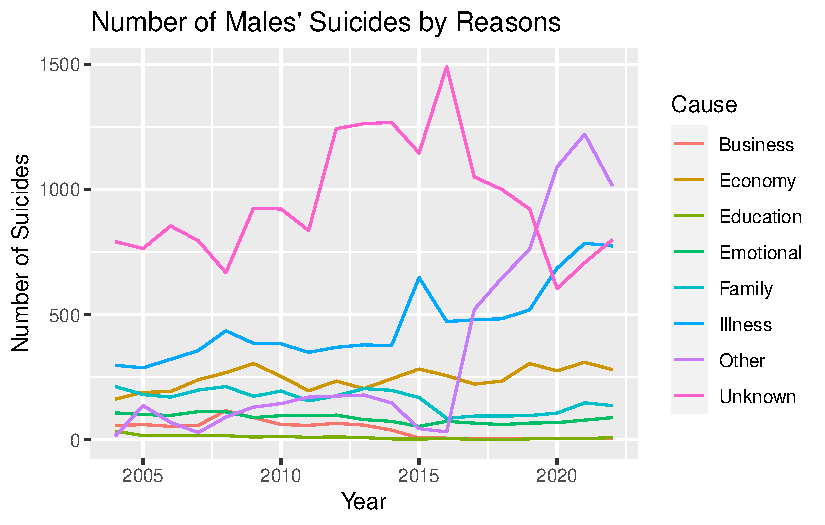
\includegraphics{analysis_files/figure-pdf/unnamed-chunk-15-1.pdf}

}

\end{figure}

\begin{Shaded}
\begin{Highlighting}[]
\NormalTok{slices }\OtherTok{=} \FunctionTok{c}\NormalTok{(}\FunctionTok{sum}\NormalTok{(}\FunctionTok{as.numeric}\NormalTok{(a1}\SpecialCharTok{$}\NormalTok{Total)),}\FunctionTok{sum}\NormalTok{(}\FunctionTok{as.numeric}\NormalTok{(a2}\SpecialCharTok{$}\NormalTok{Total)),}\FunctionTok{sum}\NormalTok{(}\FunctionTok{as.numeric}\NormalTok{(a3}\SpecialCharTok{$}\NormalTok{Total)),}\FunctionTok{sum}\NormalTok{(}\FunctionTok{as.numeric}\NormalTok{(a4}\SpecialCharTok{$}\NormalTok{Total)),}\FunctionTok{sum}\NormalTok{(}\FunctionTok{as.numeric}\NormalTok{(a5}\SpecialCharTok{$}\NormalTok{Total)),}\FunctionTok{sum}\NormalTok{(}\FunctionTok{ifelse}\NormalTok{(}\FunctionTok{is.na}\NormalTok{(}\FunctionTok{as.numeric}\NormalTok{(a6}\SpecialCharTok{$}\NormalTok{Total)),}\DecValTok{0}\NormalTok{,}\FunctionTok{as.numeric}\NormalTok{(a6}\SpecialCharTok{$}\NormalTok{Total))),}\FunctionTok{sum}\NormalTok{(}\FunctionTok{as.numeric}\NormalTok{(a7}\SpecialCharTok{$}\NormalTok{Total)),}\FunctionTok{sum}\NormalTok{(}\FunctionTok{as.numeric}\NormalTok{(a8}\SpecialCharTok{$}\NormalTok{Total)))}
\NormalTok{name }\OtherTok{=} \FunctionTok{c}\NormalTok{(}\StringTok{"Illness"}\NormalTok{,}\StringTok{"Family"}\NormalTok{,}\StringTok{"Economy"}\NormalTok{,}\StringTok{"Business"}\NormalTok{,}\StringTok{"Emotional"}\NormalTok{,}\StringTok{"Education"}\NormalTok{,}\StringTok{"Other"}\NormalTok{,}\StringTok{"Unknown"}\NormalTok{)}
\NormalTok{lbls }\OtherTok{\textless{}{-}}\NormalTok{ name}
\NormalTok{pct }\OtherTok{\textless{}{-}} \FunctionTok{round}\NormalTok{(slices}\SpecialCharTok{/}\FunctionTok{sum}\NormalTok{(slices)}\SpecialCharTok{*}\DecValTok{100}\NormalTok{)}
\NormalTok{lbls }\OtherTok{\textless{}{-}} \FunctionTok{paste}\NormalTok{(lbls, pct)}
\CommentTok{\# add percents to labels}
\NormalTok{lbls }\OtherTok{\textless{}{-}} \FunctionTok{paste}\NormalTok{(lbls,}\StringTok{"\%"}\NormalTok{,}\AttributeTok{sep=}\StringTok{""}\NormalTok{) }\CommentTok{\# ad \% to labels}
\end{Highlighting}
\end{Shaded}

\begin{Shaded}
\begin{Highlighting}[]
\FunctionTok{pie}\NormalTok{(slices,}\AttributeTok{labels =}\NormalTok{ lbls, }\AttributeTok{col=}\FunctionTok{rainbow}\NormalTok{(}\FunctionTok{length}\NormalTok{(lbls)),}
   \AttributeTok{main=}\StringTok{"Pie Chart of Males\textquotesingle{} Suicide by Reasons"}\NormalTok{,}\AttributeTok{cex=}\FloatTok{0.8}\NormalTok{)}
\end{Highlighting}
\end{Shaded}

\begin{figure}[H]

{\centering 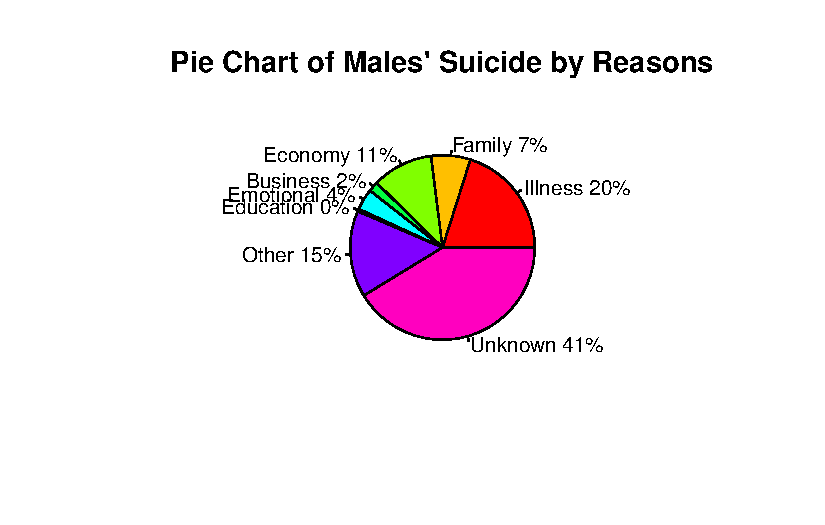
\includegraphics{analysis_files/figure-pdf/unnamed-chunk-17-1.pdf}

}

\end{figure}

\hypertarget{suicides-of-females-by-reason}{%
\subsubsection{\texorpdfstring{\textbf{Suicides of Females by
Reason}}{Suicides of Females by Reason}}\label{suicides-of-females-by-reason}}

\begin{Shaded}
\begin{Highlighting}[]
\NormalTok{  a }\OtherTok{=} \FunctionTok{filter}\NormalTok{(data,Year }\SpecialCharTok{!=} \StringTok{"2002"}\NormalTok{,Year}\SpecialCharTok{!=}\StringTok{"2003"}\NormalTok{,}\StringTok{\textasciigrave{}}\AttributeTok{Age group}\StringTok{\textasciigrave{}}\SpecialCharTok{==}\StringTok{"Total"}\NormalTok{, Sex }\SpecialCharTok{==} \StringTok{"Female"}\NormalTok{)}
\NormalTok{  a1 }\OtherTok{=} \FunctionTok{data.frame}\NormalTok{(}\AttributeTok{Year=}\NormalTok{a}\SpecialCharTok{$}\NormalTok{Year,}\AttributeTok{Total=}\NormalTok{a}\SpecialCharTok{$}\NormalTok{Illness,}\AttributeTok{Cause=}\StringTok{"Illness"}\NormalTok{)}
\NormalTok{  a2 }\OtherTok{=} \FunctionTok{data.frame}\NormalTok{(}\AttributeTok{Year=}\NormalTok{a}\SpecialCharTok{$}\NormalTok{Year,}\AttributeTok{Total=}\NormalTok{a}\SpecialCharTok{$}\StringTok{\textasciigrave{}}\AttributeTok{Family incompatibility}\StringTok{\textasciigrave{}}\NormalTok{,}\AttributeTok{Cause=}\StringTok{"Family"}\NormalTok{)}
\NormalTok{  a3 }\OtherTok{=} \FunctionTok{data.frame}\NormalTok{(}\AttributeTok{Year=}\NormalTok{a}\SpecialCharTok{$}\NormalTok{Year,}\AttributeTok{Total=}\NormalTok{a}\SpecialCharTok{$}\StringTok{\textasciigrave{}}\AttributeTok{Economic problems}\StringTok{\textasciigrave{}}\NormalTok{,}\AttributeTok{Cause=}\StringTok{"Economy"}\NormalTok{)}
\NormalTok{  a4 }\OtherTok{=} \FunctionTok{data.frame}\NormalTok{(}\AttributeTok{Year=}\NormalTok{a}\SpecialCharTok{$}\NormalTok{Year,}\AttributeTok{Total=}\NormalTok{a}\SpecialCharTok{$}\StringTok{\textasciigrave{}}\AttributeTok{Business failure}\StringTok{\textasciigrave{}}\NormalTok{,}\AttributeTok{Cause=}\StringTok{"Business"}\NormalTok{)}
\NormalTok{  a5 }\OtherTok{=} \FunctionTok{data.frame}\NormalTok{(}\AttributeTok{Year=}\NormalTok{a}\SpecialCharTok{$}\NormalTok{Year,}\AttributeTok{Total=}\NormalTok{a}\SpecialCharTok{$}\StringTok{\textasciigrave{}}\AttributeTok{Emotional relationship and not marrying the person wanted}\StringTok{\textasciigrave{}}\NormalTok{,}\AttributeTok{Cause=}\StringTok{"Emotional"}\NormalTok{)}
\NormalTok{  a6 }\OtherTok{=} \FunctionTok{data.frame}\NormalTok{(}\AttributeTok{Year=}\NormalTok{a}\SpecialCharTok{$}\NormalTok{Year,}\AttributeTok{Total=}\NormalTok{a}\SpecialCharTok{$}\StringTok{\textasciigrave{}}\AttributeTok{Educational failure}\StringTok{\textasciigrave{}}\NormalTok{,}\AttributeTok{Cause=}\StringTok{"Education"}\NormalTok{)}
\NormalTok{  a7 }\OtherTok{=} \FunctionTok{data.frame}\NormalTok{(}\AttributeTok{Year=}\NormalTok{a}\SpecialCharTok{$}\NormalTok{Year,}\AttributeTok{Total=}\NormalTok{a}\SpecialCharTok{$}\NormalTok{Other,}\AttributeTok{Cause=}\StringTok{"Other"}\NormalTok{)}
\NormalTok{  a8 }\OtherTok{=} \FunctionTok{data.frame}\NormalTok{(}\AttributeTok{Year=}\NormalTok{a}\SpecialCharTok{$}\NormalTok{Year,}\AttributeTok{Total=}\NormalTok{a}\SpecialCharTok{$}\NormalTok{Unknown,}\AttributeTok{Cause=}\StringTok{"Unknown"}\NormalTok{)}
\NormalTok{  cause }\OtherTok{=} \FunctionTok{rbind}\NormalTok{(a1,a2,a3,a4,a5,a6,a7,a8,}\AttributeTok{deparse.level =} \DecValTok{0}\NormalTok{)}
\NormalTok{  b }\OtherTok{=} \FunctionTok{as.numeric}\NormalTok{(cause}\SpecialCharTok{$}\NormalTok{Total)}
\NormalTok{  c }\OtherTok{=} \FunctionTok{ifelse}\NormalTok{(}\FunctionTok{is.na}\NormalTok{(b),}\DecValTok{0}\NormalTok{,b)}
\end{Highlighting}
\end{Shaded}

\begin{Shaded}
\begin{Highlighting}[]
\NormalTok{graph }\OtherTok{\textless{}{-}}\NormalTok{ cause }\SpecialCharTok{\%\textgreater{}\%} 
    \FunctionTok{filter}\NormalTok{(Cause }\SpecialCharTok{\%in\%} \FunctionTok{c}\NormalTok{(}\StringTok{"Illness"}\NormalTok{,}\StringTok{"Family"}\NormalTok{,}\StringTok{"Economy"}\NormalTok{,}\StringTok{"Business"}\NormalTok{,}\StringTok{"Emotional"}\NormalTok{,}\StringTok{"Education"}\NormalTok{,}\StringTok{"Other"}\NormalTok{,}\StringTok{"Unknown"}\NormalTok{))}
\NormalTok{  graph }\SpecialCharTok{\%\textgreater{}\%}
    \FunctionTok{ggplot}\NormalTok{( }\FunctionTok{aes}\NormalTok{(}\AttributeTok{x=}\NormalTok{Year, }\AttributeTok{y=}\NormalTok{c, }\AttributeTok{group=}\NormalTok{Cause, }\AttributeTok{color=}\NormalTok{Cause)) }\SpecialCharTok{+}
      \FunctionTok{geom\_line}\NormalTok{() }\SpecialCharTok{+}
      \FunctionTok{ylab}\NormalTok{(}\StringTok{"Number of Suicides"}\NormalTok{) }\SpecialCharTok{+}
      \FunctionTok{ggtitle}\NormalTok{(}\StringTok{"Number of Females\textquotesingle{} Suicide by Reasons"}\NormalTok{)}
\end{Highlighting}
\end{Shaded}

\begin{figure}[H]

{\centering 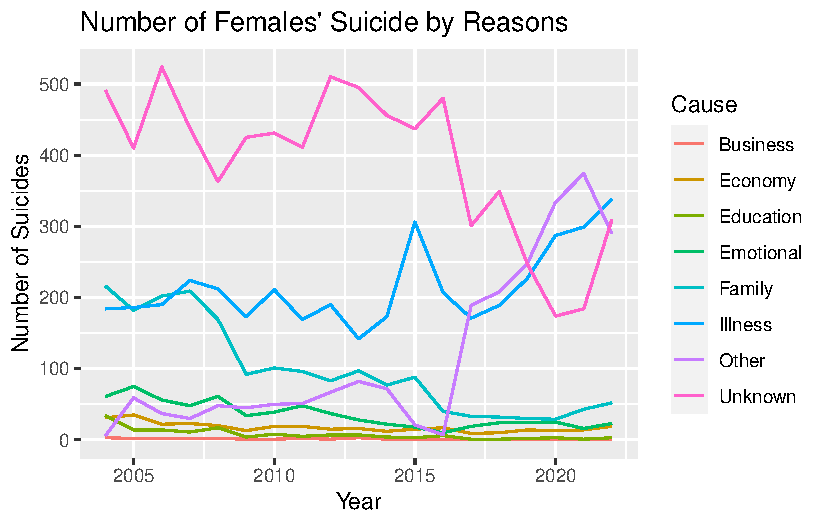
\includegraphics{analysis_files/figure-pdf/unnamed-chunk-19-1.pdf}

}

\end{figure}

\begin{Shaded}
\begin{Highlighting}[]
\NormalTok{slices }\OtherTok{=} \FunctionTok{c}\NormalTok{(}\FunctionTok{sum}\NormalTok{(}\FunctionTok{as.numeric}\NormalTok{(a1}\SpecialCharTok{$}\NormalTok{Total)),}\FunctionTok{sum}\NormalTok{(}\FunctionTok{as.numeric}\NormalTok{(a2}\SpecialCharTok{$}\NormalTok{Total)),}\FunctionTok{sum}\NormalTok{(}\FunctionTok{as.numeric}\NormalTok{(a3}\SpecialCharTok{$}\NormalTok{Total)),}\FunctionTok{sum}\NormalTok{(}\FunctionTok{ifelse}\NormalTok{(}\FunctionTok{is.na}\NormalTok{(}\FunctionTok{as.numeric}\NormalTok{(a4}\SpecialCharTok{$}\NormalTok{Total)),}\DecValTok{0}\NormalTok{,}\FunctionTok{as.numeric}\NormalTok{(a4}\SpecialCharTok{$}\NormalTok{Total))),}\FunctionTok{sum}\NormalTok{(}\FunctionTok{ifelse}\NormalTok{(}\FunctionTok{is.na}\NormalTok{(}\FunctionTok{as.numeric}\NormalTok{(a5}\SpecialCharTok{$}\NormalTok{Total)),}\DecValTok{0}\NormalTok{,}\FunctionTok{as.numeric}\NormalTok{(a5}\SpecialCharTok{$}\NormalTok{Total))),}\FunctionTok{sum}\NormalTok{(}\FunctionTok{ifelse}\NormalTok{(}\FunctionTok{is.na}\NormalTok{(}\FunctionTok{as.numeric}\NormalTok{(a6}\SpecialCharTok{$}\NormalTok{Total)),}\DecValTok{0}\NormalTok{,}\FunctionTok{as.numeric}\NormalTok{(a6}\SpecialCharTok{$}\NormalTok{Total))),}\FunctionTok{sum}\NormalTok{(}\FunctionTok{as.numeric}\NormalTok{(a7}\SpecialCharTok{$}\NormalTok{Total)),}\FunctionTok{sum}\NormalTok{(}\FunctionTok{as.numeric}\NormalTok{(a8}\SpecialCharTok{$}\NormalTok{Total)))}
\NormalTok{name }\OtherTok{=} \FunctionTok{c}\NormalTok{(}\StringTok{"Illness"}\NormalTok{,}\StringTok{"Family"}\NormalTok{,}\StringTok{"Economy"}\NormalTok{,}\StringTok{"Business"}\NormalTok{,}\StringTok{"Emotional"}\NormalTok{,}\StringTok{"Education"}\NormalTok{,}\StringTok{"Other"}\NormalTok{,}\StringTok{"Unknown"}\NormalTok{)}
\NormalTok{lbls }\OtherTok{\textless{}{-}}\NormalTok{ name}
\NormalTok{pct }\OtherTok{\textless{}{-}} \FunctionTok{round}\NormalTok{(slices}\SpecialCharTok{/}\FunctionTok{sum}\NormalTok{(slices)}\SpecialCharTok{*}\DecValTok{100}\NormalTok{)}
\NormalTok{lbls }\OtherTok{\textless{}{-}} \FunctionTok{paste}\NormalTok{(lbls, pct)}
\CommentTok{\# add percents to labels}
\NormalTok{lbls }\OtherTok{\textless{}{-}} \FunctionTok{paste}\NormalTok{(lbls,}\StringTok{"\%"}\NormalTok{,}\AttributeTok{sep=}\StringTok{""}\NormalTok{) }\CommentTok{\# ad \% to labels}
\end{Highlighting}
\end{Shaded}

\begin{Shaded}
\begin{Highlighting}[]
\FunctionTok{pie}\NormalTok{(slices,}\AttributeTok{labels =}\NormalTok{ lbls, }\AttributeTok{col=}\FunctionTok{rainbow}\NormalTok{(}\FunctionTok{length}\NormalTok{(lbls)),}
   \AttributeTok{main=}\StringTok{"Pie Chart of Females\textquotesingle{} Suicide by Reasons"}\NormalTok{,}\AttributeTok{cex=}\FloatTok{0.8}\NormalTok{)}
\end{Highlighting}
\end{Shaded}

\begin{figure}[H]

{\centering 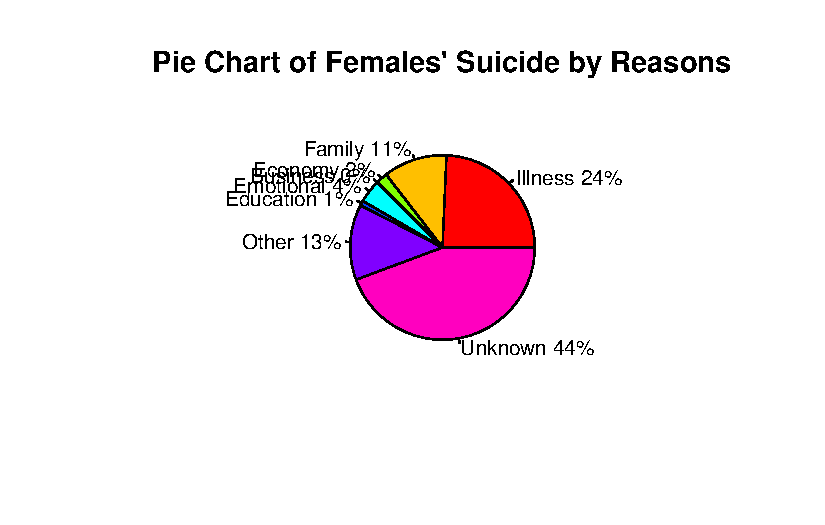
\includegraphics{analysis_files/figure-pdf/unnamed-chunk-21-1.pdf}

}

\end{figure}



\end{document}
